\section{PHƯƠNG TRÌNH ĐƯỜNG THẲNG}
\subsection{LÝ THUYẾT CẦN NHỚ}
\subsubsection{Phuơng trình tổng quát của đường thẳng}
\begin{itemize}
	\immini{
		\item[\iconMT]\indam{Véc tơ pháp tuyến:} Véc-tơ $\overrightarrow{n} \ne \vec{0}$ được gọi là véc-tơ pháp tuyến (vtpt) của đường thẳng $\Delta $ nếu giá của $\overrightarrow{n}$ vuông góc với $\Delta $ (hình vẽ).\\
		\begin{tcolorbox}[colframe=orange,colback=orange!4!,boxrule=0.2mm]
			\begin{itemize}
				\item  Một đường thẳng có vô số véc-tơ pháp tuyến và chúng cùng phương nhau.
				\item  Nếu $\overrightarrow{n}$ và $\overrightarrow{n'}$ cùng là véc-tơ pháp tuyến của $\Delta$ thì $\overrightarrow{n'}$=$k \cdot \overrightarrow{n}$.
				\item  Đường thẳng $\Delta$ hoàn toàn xác định khi biết một điểm và một véc tơ pháp tuyến của nó.
			\end{itemize}
		\end{tcolorbox}
	}{
		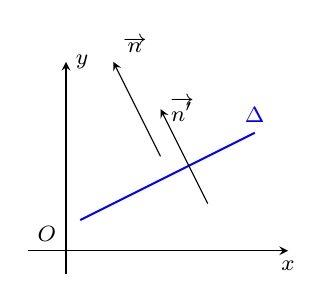
\begin{tikzpicture}[smooth,samples=300,scale=0.6,>=stealth,font=\footnotesize]
			\draw[->] (-0.8,0)--(4.7,0) node[below]{$x$};
			\draw[->] (0,-0.5)--(0,4) node[right]{$y$};
			\draw (0,0) node[above left]{$O$};
			\draw[line width=0.7pt, blue,domain=0.3:4] plot(\x,{0.5*((\x)+1)})node[above]{$\Delta$};
			\draw[->] (2,2)--(1,4) node[above right]{$\overrightarrow{n}$};
			\draw[->] (3,1)--(2,3) node[right]{$\overrightarrow{n'}$};
	\end{tikzpicture}}
	\item [\iconMT] \indam{Phương trình tổng quát của đường thẳng:} \\
	\begin{minipage}[b]{8cm}
		\begin{itemize}
		\item [\ding{172}] Đường thẳng $\Delta \colon \heva{& \text{ qua } M(x_0;y_0) & (1)\\& \text{vtpt } \overrightarrow{n}=\left(a;b\right)& (2)}$ sẽ có phương trình tổng quát là 
		\boxmini{$a(x-x_0)+b(y-y_0)=0$ \quad $(\star)$}
		ta thu gọn $(\star)$ về dạng $ax+by+c=0$.
		\item [\ding{173}] Cho $\Delta \colon ax+by+c=0$. 
		\begin{itemize}
			\item [$\bullet$] Nếu $b=0$ thì $\Delta$ có thể đưa về dạng $x=-\dfrac{c}{a}$ (vuông góc với $Ox$).
			\item [$\bullet$] Nếu $b \ne 0$, chia hai vế cho $b$ thì $\Delta$ có thể đưa về dạng $y=-\dfrac{a}{b}x-\dfrac{c}{b}$.
		\end{itemize}
	\end{itemize}
	\end{minipage}\hspace{2cm}
\begin{minipage}[b]{6cm}
\hspace*{1cm}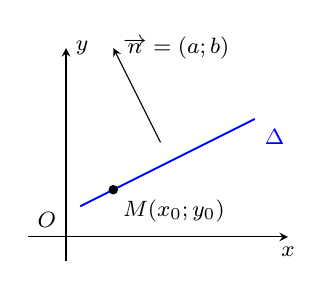
\begin{tikzpicture}[smooth,samples=300,scale=0.6,>=stealth,font=\footnotesize]
	\draw[->] (-0.8,0)--(4.7,0) node[below]{$x$};
	\draw[->] (0,-0.5)--(0,4) node[right]{$y$};
	\draw (0,0) node[above left]{$O$};
	\draw[line width=0.7pt, blue,domain=0.3:4] plot(\x,{0.5*((\x)+1)})node[below right]{$\Delta$};
	\draw[->] (2,2)--(1,4) node[right]{$\overrightarrow{n}=(a;b)$};
	\draw[fill=black] (1,1) circle (2.5pt) node[below right]{$M(x_0;y_0)$};
\end{tikzpicture}\\
	\begin{khung4}{Chú ý}
	Để viết được phương trình tổng quát của đường thẳng $\Delta$, ta cần xác định được hai dữ kiện (1) và (2), sau đó áp dụng công thức $(\star)$ và thu gọn kết quả.
\end{khung4}
%\vspace{3cm}
\end{minipage}
\end{itemize}

\subsubsection{ Phương trình tham số của đường thẳng}
\begin{itemize}
	\immini{\item [\iconMT] \indam{Véc tơ chỉ phương: }Véc-tơ $\overrightarrow{u} \ne \vec{0}$ được gọi là véc-tơ chỉ phương (vtcp) của đường thẳng $\Delta $ nếu giá của $\overrightarrow{u}$ song song hoặc trùng với $\Delta $.\\
		\begin{tcolorbox}[colframe=orange,colback=orange!4!,boxrule=0.2mm]
			\begin{itemize}
				\item  Một đường thẳng có vô số véc-tơ chỉ phương và chúng cùng phương với nhau.	
				\item  Đường thẳng $\Delta$ hoàn toàn xác định khi biết một điểm và một véc tơ chỉ phương của nó.
			\end{itemize}
		\end{tcolorbox}
		}{\hspace{1cm}
		\begin{tikzpicture}[smooth,samples=300,scale=0.7,>=stealth,font=\footnotesize]
			\draw[->] (-0.8,0)--(5,0) node[below]{$x$};
			\draw[->] (0,-0.5)--(0,4) node[right]{$y$};
			\draw (0,0) node[above left]{$O$};
			\draw[magenta,line width=0.7pt,domain=0.3:4] plot(\x,{0.5*((\x)+1)})node[above]{$\Delta$};
			\draw[->,blue] (1,2)--(3,3) node[above]{$\overrightarrow{u}$};
			\draw[->,violet] (1,0.5)--(4,2) node[below right]{$\overrightarrow{u'}$};
			\node[below] at (2,-1.3) {Nếu $\overrightarrow{u}$ và $\overrightarrow{u'}$ là véc-tơ chỉ phương}; 
			\node[below] at (2,-2.3) {của $\Delta$ thì $\overrightarrow{u}=k \cdot \overrightarrow{u}$.}; 
	\end{tikzpicture}
\vspace{-1cm}
}
\indamm{Mối liên hệ giữa véc tơ chỉ phương và véc tơ pháp tuyến:} Cho $\vec{n}=(a;b)$ là một véc tơ pháp tuyến của $\Delta$. Khi đó $\Delta$ có một véc tơ chỉ phương là $\vec{u}=(-b;a)$ hoặc $\vec{u}=(b;-a)$.
\item[\iconMT] \indam{Phương trình tham số của đường thẳng:} Đường thẳng $\Delta \colon \heva{& \text{ qua } M(x_0;y_0) & (1)\\& \text{vtcp } \overrightarrow{u}=\left(u_1;u_2\right)& (2)}$ sẽ có phương trình tham số là \boxmini{$\heva{&x=x_0+u_1t\\&y=y_0+u_2t}\quad (t \in \mathbb{R})$}
\end{itemize}

\subsubsection{Mối liên hệ giữa đồ thị hàm bậc nhất và đường thẳng}
\begin{listEX}[1]
	\item [\ding{172}] Đồ thị hàm số bậc nhất $y=kx+y_0$ là một đường thẳng có hệ số góc $k$ có thể được viết thành $kx-y+y_0$. Suy ra một véc tơ pháp tuyến là $\vec{n}=(k;-1)$.
	\begin{boxdn}
		\indam{Ghi nhớ:} Một đường thẳng có hệ số góc $k$ thì nó sẽ có một véc tơ pháp tuyến là $\vec{n}=(k;-1)$.
	\end{boxdn}
	\item [\ding{173}] Ngược lại, mỗi đường thẳng có phương trình $ax+by+c=0$, với $a,\,b \ne 0$ có thể được viết thành dạng hàm số bậc nhất $y=-\dfrac{a}{b}x-\dfrac{c}{b}$.
\end{listEX}
\subsection{RÈN LUYỆN KĨ NĂNG GIẢI TOÁN}

\begin{dang}{Phương trình tổng quát của đường thẳng}
	\indam{Xét phương trình tổng quát:} Cho $\Delta \colon ax+by+c=0$ thì
	\begin{itemize}
		\item [$\bullet$] Một vtpt là $\overrightarrow{n}=(a,b)$ (hệ số của $x$ và $y$.)
		\item [$\bullet$] Tìm điểm thuộc $\Delta$: Cho trước $x$, thay vào phương trình tìm $y$ hoặc ngược lại.
	\end{itemize}
\end{dang}
\begin{vd}
	Trong mặt phẳng $Oxy$, cho đường thẳng $\Delta \colon 2x-y+5=0$.
	\begin{tasks}(1)
		\task Tìm một điểm thuộc $\Delta$ và một vec tơ pháp tuyến của $\Delta$.
		\task Gọi $M(x_1;y_1)$ và $N(x_2;y_2)$ thuộc $\Delta$. Tính độ dài đoạn $MN$, biết $x_1=4$ và $x_2=1$.
	\end{tasks}
	\loigiai{
		\begin{tasks}(1)
			\task Cho $x=0$, ta được $y=5$. Vậy $M(0;5)\in \Delta$. \\
			Xét hệ số của $x$ và $y$, suy ra một véc-tơ pháp tuyến là $\vec{n}=(2;-1)$.
			\task Với $x_1=4$ thì $2 \cdot 4 -y+5=0 \Rightarrow y=13$. Suy ra $M(4;13)$.\\
			Với $x_2=1$ thì $2 \cdot 1 - y +5 =0 \Rightarrow y=7$. Suy ra $N(1;7$.\\
			Vậy $MN=\sqrt{(1-4)^2+(7-13)^2}=3\sqrt{5}$.
	\end{tasks}}
	
\end{vd}\dongcham{6}

\begin{vd}
	Trong mặt phẳng $Oxy$, viết phương trình tổng quát đường thẳng $\Delta$ đi qua điểm $M(-1;5)$ và có véc-tơ pháp tuyến $ \overrightarrow{n} = \left(-2;3 \right)$.
	\loigiai{
		Phương trình đường thẳng $\Delta:$ $ -2 ( x + 1) + 3( y - 5) = 0 \Leftrightarrow -2x + 3y - 17 =0$.\\
		Vậy phương trình tổng quát đường thẳng $\Delta: -2x + 3y - 17 =0$.
	}
\end{vd}\dongcham{6}

\begin{vd}
	Lập phương trình tổng quát của đường thẳng qua điểm $M(-2;3)$ và có hệ số góc $k=2$.
	\loigiai{
	Hệ số góc $k=2$, suy ra một véc tơ pháp tuyến là $\vec{n}=(2;-1)$.\\
	Phương trình đường thẳng cần tìm là $2(x+2)-1(y-3)=0\Leftrightarrow 2x-y+7=0$.}
\end{vd}\dongcham{6}
\begin{vd}
	Trong mặt phẳng $Oxy$ cho tam giác $ABC$ với $A(1;-2)$, $B(2;0)$, $C(2;4)$. 
	\begin{tasks}(1)
		\task Lập phương trình đường cao kẻ từ $A$ và đường cao kẻ từ $B$ của tam giác $ABC$.
		\task Lập phương trình đường trung trực cạnh $BC$ và trung trực cạnh $AC$.
	\end{tasks}
\loigiai{
}
\end{vd}\dongcham{12}

\begin{dang}{Phương trình tham số của đường thẳng}
	\indam{Xét phương trình tham số:} Cho $\Delta \colon \heva{&x=x_0+u_1t\\&y=y_0+u_2t}$ thì
	\begin{itemize}
		\item [$\bullet$] Một vtcp là $\overrightarrow{u}=(u_1;u_2)$ (hệ số của $t$.)
		\item [$\bullet$] Tìm điểm thuộc $\Delta$: Cho trước $t$, thay vào phương trình tìm $x$ và $y$.
	\end{itemize}

\end{dang}
\begin{vd}
	Trong mặt phẳng $Oxy$, cho đường thẳng $\Delta \colon \heva{&x=1-3t\\&y=2+t}$.
	\begin{tasks}(1)
		\task Tìm một điểm thuộc $\Delta$ và một véc tơ chỉ phương của $\Delta$.
		\task Gọi $M(x_1;y_1)$ và $N(x_2;y_2)$ thuộc $\Delta$. Tính độ dài đoạn $MN$, biết $x_1=4$ và $x_2=1$.
	\end{tasks}
	\loigiai{
		\begin{tasks}(1)
			\task Cho $t=0$, ta được $x=1$, $y=2$. Vậy $M(1;2)\in \Delta$. \\
			Xét hệ số của $t$, suy ra một véc-tơ chỉ phương là $\vec{u}=(-3;1)$.
			\task Với $x_1=4$ thì $1-3t=4 \Rightarrow t=-1$. Suy ra $M(4;1)$.\\
			Với $x_2=1$ thì $1-3t=1 \Rightarrow t=0$. Suy ra $N(1;2)$.\\
			Vậy $MN=\sqrt{(1-4)^2+(2-1)^2}=\sqrt{10}$.
		\end{tasks}
	}
	
\end{vd}\dongcham{5}
\begin{vd}
	Trong mặt phẳng $Oxy$, viết phương trình tham số đường thẳng $\Delta$ biết $\Delta$ đi qua $M(1;2)$ và có vec-tơ chỉ phương $ \overrightarrow{u} = (-1;3)$.
	\loigiai{
		Phương trình tham số đường thẳng $\Delta$: $\left\{ \begin{array}{l} x = 1 - t \\ y = 2 + 3t\end{array} \right.$.
	}
\end{vd}\dongcham{4}

\begin{vd}
	Trong mặt phẳng $Oxy$, lập phương trình tham số của đường thẳng $d $ đi qua điểm $M(5;1)$ và có hệ số góc $k=8.$ 
	\loigiai{ 
		$d$ có hệ số góc $k=8$ nên có VTCP $\overrightarrow{u}=(1;8).$ \\
		Vậy phương trình tham số của $d$ là: $\left\{\begin{aligned}& x=5+t \\ & y=1+8t. \\ \end{aligned}\right. $ 
	}
\end{vd}\dongcham{4}

\begin{vd}
	Trong mặt phẳng $Oxy$, cho tam giác $ABC$ với $A(1;-2)$, $B(2;0)$, $C(2;4)$. 
	\begin{tasks}(1)
		\task Lập phương trình đường thẳng đi qua $A$ và song song với $BC$.
		\task Lập phương trình tham số của đường trung bình tam giác ứng với cạnh đáy $ BC$.
	\end{tasks}
	\loigiai{
	}
\end{vd}\dongcham{10}

\begin{dang}{Chuyển phương trình tham số về phương trình tổng quát và ngược lại}
	\indam{Mối liên hệ giữa véc tơ chỉ phương và véc tơ pháp tuyến:} Cho $\vec{n}=(a;b)$ là một véc tơ pháp tuyến của $\Delta$. Khi đó $\Delta$ có một véc tơ chỉ phương là $\vec{u}=(-b;a)$ hoặc $\vec{u}=(b;-a)$ (đổi chỗ và đổi 1 dấu).
\end{dang}

\begin{vd}
	Trong mặt phẳng $Oxy$, cho đường thẳng $\Delta \colon \heva{&x=2+3t\\&y=4-t}$. Viết phương trình tổng quát của đường thẳng $\Delta$.
	\loigiai{
		$\Delta$ qua $M(2;4)$ và có vtcp $\vec{u}=(3;-1)$. Suy ra $\vec{n}=(1;3)$ là vtpt của $\Delta$.\\
		Phương trình tổng quát của $\Delta$ là
		$$1(x-2)+3(y-4)=0 \Leftrightarrow x+3y-14=0.$$
		
	}
\end{vd}\dongcham{5}

\begin{vd}
	Trong mặt phẳng $Oxy$, cho đường thẳng $\Delta \colon 3x - 4y + 4=0$. Lập phương trình tham số của $\Delta$.
	\loigiai{
		$\Delta$ qua $M(0;1)$ và có vtpt $\vec{n}=(3;-4)$. Suy ra, vtcp của $\Delta$ là $\vec{u}=(4;3)$.\\
		Phương trình tham số của $\Delta$ là $\heva{&x=4t\\&1+3t}$.}
\end{vd}\dongcham{5}

\begin{dang}{Lập phương trình đường thẳng đi qua hai điểm phân biệt cho trước}
	\begin{itemize}
		\item [\iconMT] Trong mặt phẳng $Oxy$, cho hai điểm $A(x_A;y_A)$ và $B(x_B;y_B)$. Khi đó, đường thẳng $AB$ sẽ có một véc tơ chỉ phương là $\vec{AB}=(x_B-x_A;y_B-y_A)$.
		\item [\iconMT] \indam{Lưu ý:}
		\begin{itemize}
			\item [$\bullet$] Nếu $x_B-x_A \ne 0$ và $y_B-y_A \ne 0$ thì phương trình $AB$ là
			$\dfrac{x-x_A}{x_B-x_A}=\dfrac{y-y_A}{y_B-y_A}$.
			\item [$\bullet$] Nếu $A(a;0)$ và $B(0;b)$, với $a,b \ne 0$ thì phương trình $AB$ là $\dfrac{x}{a}+\dfrac{y}{b}=1$.
		\end{itemize}
	\end{itemize}
\end{dang}
\begin{vd}
	Trong mặt phẳng $Oxy$,  lập phương trình tham số và phương trình tổng quát của đường thẳng $d$ đi qua $A \left(1; 2 \right), B \left(3;1 \right)$.
	\loigiai{
		\begin{itemize}
			\item [\iconMT] Đường thẳng $d$ qua $A \left(1;2 \right)$ và nhận $\overrightarrow{AB} = (2;-1)$ làm véc-tơ chỉ phương. \\
			Vậy phương trình tham số đường thẳng $d$: $\left\{ \begin{array}{l} x = 1 + 2t \\ y = 2 - t\end{array} \right.$.
			\item [\iconMT] Véc tơ pháp tuyến của $d$ là $\vec{n}=(1;2)$. Phương trình tổng quát của $d$ là
			$$1(x-1)+2(y-2)=0 \Leftrightarrow x+2y-5=0$$
		\end{itemize}
		
	}
\end{vd}\dongcham{6}

\begin{vd}
	Trong mặt phẳng $Oxy$, cho tam giác $ABC$ với $A(1;2)$, $B(3;0)$, $C(1;4)$.
	\begin{tasks}(1)
		\task Viết phương trình tổng quát của các đường thẳng chứa các cạnh của tam giác $ABC$.
		\task Viết phương trình tham số và phương trình tổng quát của đường trung tuyến kẻ từ $A$.
	\end{tasks}
	\loigiai{}
\end{vd}\dongcham{12}

\begin{vd}%[0H3K1-2]  
	Một đường thẳng đi qua điểm $M(5;-3)$ cắt trục $Ox$ và $Oy$ tại $A$ và $B$ sao cho $M$ là trung điểm của $AB$. Viết phương trình tổng quát của đường thẳng đó.
	\loigiai{ 
		Giả sử $A=(a;0),B=(0;b) $. Vì $M(5;-3)$ là trung điểm của $AB$ nên
		$$\heva{5=\dfrac{a+0}{2}\\-3=\dfrac{0+b}{2}} \Rightarrow \heva{&a=10\\&b=-6.}$$
		Phương trình của đường thẳng đi qua $A,B$ là $\dfrac{x}{10}+\dfrac{y}{-6}=1$ hay $3x-5y-30=0$.
	}
\end{vd}\dongcham{10}  

\begin{vd}%[0H3K1-7]
	\immini{
		Để tham gia một phòng tập thể dục, người tập phải trả một khoản phí tham gia ban đầu và phí sử dụng phòng tập. Đường thẳng $\Delta$ ở hình bên biểu thị tổng chi phí (đơn vị: triệu đồng) tham gia một phòng tập thể dục theo thời gian tập của một người (đơn vị: tháng).
		\begin{enumerate}
			\item Viết phương trình của đường thẳng $\Delta$.
			\item Cho biết giao điểm của đường thẳng $\Delta$ với trục tung trong tình huống này có ý nghĩa gì?
			\item Tính tổng chi phí mà người đó phải trả khi tham gia phòng tập thể dục với thời gian $12$ tháng.
		\end{enumerate}
	}{
		\begin{tikzpicture}[scale=0.7, font=\footnotesize, line join=round, line cap=round, >=stealth,x=0.7cm,y=0.7cm]
			\draw[->](0,-0.5)--(0,8.5) node[left]{$y$};
			\draw[->](-0.5,0)--(13,0) node[above]{$x$};
			\draw (0,0) node [below left] {$O$};
			\foreach \x in {1,2,3,...,12}
			\draw[shift={(\x,0)},color=black] (0pt,2pt) -- (0pt,-2pt);
			\foreach \y in {1,2,3,...,8}
			\draw[shift={(0,\y)},color=black] (2pt,0pt) -- (-2pt,0pt);
			\draw[fill=black] (0,1.5) circle (1pt) node[left] {$1.5$} (7,5) circle (1pt);
			\draw[dashed] (7,0) node[below]{$7$}--(7,5)--(0,5) node[left]{$5$};
			\draw (1,0) node[below]{$1$} (12,0) node[below]{$12$}
			(0,1) node[left]{$1$} (12,8)node{$\Delta$};
			\draw (6,-1.5) node{Tháng} (-3,4) node[rotate=90]{Chi phí (triệu đồng)};
			\draw[samples=100,smooth,domain=0:12] plot (\x,{0.5*(\x)+1.5});
		\end{tikzpicture} 
	}
	\loigiai{
		\begin{enumerate}
			\item Đường thẳng $\Delta$ đi qua hai điểm lần lượt có tọa độ $(0 ; 1.5)$ và $(7 ; 5)$ nên $\Delta$ có phương trình là
			\begin{eqnarray*}
				& & \dfrac{x-0}{7-0}=\dfrac{y-1.5}{5-1.5} \Leftrightarrow \dfrac{x}{7} = \dfrac{y-1.5}{3.5}\\
				& \Leftrightarrow & \dfrac{x}{7}=\dfrac{2y-3}{7} \Leftrightarrow x=2y-3\\
				& \Leftrightarrow & y = \dfrac{1}{2}x+\dfrac{3}{2}.
			\end{eqnarray*}
			\item Giao điểm của đường thẳng $\Delta$ với trục $O y$ ứng với $x=0$. \\
			Thời điểm $x=0$ cho biết mức phí ban đầu lắp đặt để sử dụng phòng tập. \\
			Khi $x=0$ thì $y=1.5$, vì vậy chi phí tham gia phòng tập ban đầu là $1{,}5$ triệu đồng.
			\item $12$ tháng đầu tiên ứng với $x=12$. Do đó: $y=\dfrac{1}{2}\cdot12+\dfrac{3}{2}=7{,}5$.\\
			Vậy tổng chi phí tham gia và sử dụng phòng tập trong $12$ tháng đầu tiên là $7{,}5$ triệu đồng.
		\end{enumerate}
	}
\end{vd}\dongcham{15}

\subsection{BÀI TẬP TỰ LUYỆN}

\begin{baitap}
	Viết phương trình tham số và phương trình tổng quát của trục $Ox$, trục $Oy$.
\end{baitap}\cham{6}

\begin{baitap}%[Tex hóa SGK CD-CT,T7/22, Lê Minh Thiện Anh]%[0H3Y1-2]
	Lập phương trình tổng quát và phương trình tham số của đường thẳng $d$ trong mỗi trường hợp sau:
	\begin{enumEX}[a)]{1}
	\item $d$ đi qua điểm $M(2;2)$ và có véc-tơ chỉ phương $\overrightarrow{u}=(4;7)$;
	\item d đi qua điểm $N(0;1)$ và có véc-tơ pháp tuyến là $\overrightarrow{n}=(-5;3)$;
	\item $d$ đi qua $A(-2;-3)$ và có hệ số góc $k=3$;
	\item $d$ đi qua hai điểm $P(1;1)$ và $Q(3;4)$.
	\end{enumEX}
	\loigiai{
		\begin{enumerate}
			\item Phương trình tham số của $d$ là: $\heva{&x=2+4t\\&y=2+7t.}$\\
			Phương trình tổng quát của $d$ là: $7x-4y-6=0$.
			\item Véc-tơ pháp tuyến là $\overrightarrow{n}=(-5;3) \Rightarrow$ véc-tơ chỉ phương là $\overrightarrow{u}=(3;5)$.\\
			Phương trình tham số của $d$ là: $\heva{&x=3t\\&y=1+5t.}$\\
			Phương trình tổng quát của $d$ là: $5x-3y+3=0$.
			\item Phương trình tổng quát của $d$ là: $y+3=3(x+2) \Leftrightarrow 3x-y+3=0$.\\
			Phương trình tham số của $d$ là: $\heva{&x=t\\&y=3+3t.}$
			\item Véc-tơ chỉ phương là $\overrightarrow{u}=\overrightarrow{PQ}=(2;3) \Rightarrow$ véc-tơ pháp tuyến là $\overrightarrow{n}=(3;-2)$.\\
			Phương trình tổng quát của $d$ là: $3 \cdot (x-1)-2$. $(y-1)=0 \Leftrightarrow 3x-2y-1=0$.\\
			Phương trình tham số của $d$ là: $\heva{&x=1+2t\\&y=1+3t.}$.
		\end{enumerate}
	}
\end{baitap}\cham{25}

\begin{baitap}%[Tex hóa SGK CD,T8/22, Phạm Doãn Lê Bình]%[0H3B1-2]
	Cho đường thẳng $d$ có phương trình tham số là $\heva{& x=-1-3 t \\ & y=2+2 t.}$
	\begin{enumerate}
		\item Lập phương trình tổng quát của đường thẳng $d$.
		\item Tìm toạ độ giao điểm của đường thẳng $d$ lần lượt với các trục $O x, O y$.
		\item Đường thẳng $d$ có đi qua điểm $M(-7 ; 5)$ hay không?
	\end{enumerate}
	\loigiai{
		\begin{enumerate}
			\item Từ phương trình tham số của đường thẳng $d$ ta suy ra $d$ đi qua điểm $A(-1;2)$ và có một véc-tơ chỉ phương $\vec{u}=(-3;2)$ nên $d$ có một véc-tơ pháp tuyến $\vec{n}=(2;3)$. \\
			Phương trình tổng quát của đường thẳng $d$ là
			\[ 2(x+1)+3(y-2)=0 \Leftrightarrow 2x+3y-4=0.\]
			\item Thay $y=0$ vào phương trình của $d$ ta có $2x+3\cdot 0 -4=0 \Leftrightarrow x = 2$. Vậy đường thẳng $d$ cắt trục $Ox$ tại điểm $B(2;0)$.\\
			Thay $x=0$ vào phương trình của $d$ ta có $2\cdot 0+3y -4=0 \Leftrightarrow y = \dfrac{4}{3}$. Vậy đường thẳng $d$ cắt trục $Oy$ tại điểm $C\left(0;\dfrac{4}{3}\right)$.
			\item Thay $x=-7$ vào phương trình của $d$ ta có $2\cdot (-7)+3y -4=0 \Leftrightarrow y = 6$. Vậy đường thẳng $d$ không đi qua điểm $M(-7;5)$.
		\end{enumerate}
	}
\end{baitap}\cham{9}

\begin{baitap}
	Trong mặt phẳng tọa độ, cho tam giác $ ABC$ với $ A\left(1;4\right)$, $B\left(3;-1\right)$, $C\left(6;2\right)$.
\begin{enumEX}[a)]{1}
	\item Lập phương trình tổng quát của đường cao $ AH$ tam giác $ ABC$.
	\item Lập phương trình tham số của đường thẳng $ d$ đi qua $ B$ và song song với $ AC$.
	\item Lập phương trình tham số của đường trung bình tam giác ứng với cạnh đáy $ BC$.
	\item Lập phương trình tổng quát đường trung tuyến kẻ từ $A$.
\end{enumEX}
\loigiai{
	\begin{enumEX}[a)]{1}
		\item Đường thẳng cao $ AH$ tam giác $ ABC$ là đường thẳng đi qua $ A\left(1;4\right)$ và có một vectơ pháp tuyến là $\overrightarrow{BC}=\left(3;3\right)$.\\
		Do đó, đường thẳng cao $ AH$ tam giác $ ABC$ có phương trình tổng quát là
		$$ 3.\left(x-1\right)+3.\left(y-4\right)=0\Leftrightarrow x+y-5=0.$$
		\item Đường thẳng $ d$ đi qua $ B\left(3;-1\right)$ và song song với $ AC$ nhận $\overrightarrow{AC}=\left(5;-2\right)$ là vectơ chỉ phương.\\
		Vậy phương trình tham số của đường thẳng $ d$ là $\heva{&x=3+5t\\&y=-1-2t}$.
		\item Đường trung bình tam giác $ ABC$ ứng với cạnh đáy $ BC$ là đường thẳng qua trung điểm $ M\left(2;\dfrac{3}{2}\right)$ của cạnh $ AB$ và song song với $ BC$ hay có một vectơ chỉ phương là $\overrightarrow{BC}=\left(3;3\right)$ hay $\overrightarrow u=\left(1;1\right)$.\\
		Vậy phương trình tham số của đường trung bình tam giác $ ABC$ ứng với cạnh đáy $ BC$ là $\heva{&x=2+t\\&y=1.5+t}$.
	\end{enumEX}
}
\end{baitap}\cham{32}

\begin{baitap}
	Trong mặt phẳng $Oxy$, cho tam giác $ABC$ biết $A(2;1),B(-1;0),C(0;3)$.
\begin{enumEX}[a)]{1}
		\item Viết phương trình tổng quát của đường cao $AH$.
		\item Viết phương trình tổng quát đường trung trực của đoạn thẳng $AB$.
		\item Viết phương trình tổng quát đường thẳng $BC$.
		\item Viết phương trình tổng quát đường thẳng qua $A$ và song song với đường $BC$.
		\item Viết phương trình tổng quát đường trung tuyến kẻ từ $A$.
\end{enumEX}
	\loigiai{ 
		\begin{enumerate}
			\item Ta có đường cao $AH$ đi qua $A$ và nhận $\overrightarrow{BC}(1;3)$ là vtpt nên có phương trình tổng quát là $1.(x-2)+3.(y-1)=0$ hay $x+3y-5=0$.
			\item Gọi $I$ là trung điểm $AB$ khi đó $x_I=\dfrac{x_B+x_C}{2}=\dfrac{1}{2},y_I=\dfrac{y_B+y_C}{2}=\dfrac{1}{2} \Rightarrow I\left(\dfrac{1}{2};\dfrac{1}{2}\right).$ \\
			Đường trung trực đoạn thẳng $AB$ đi qua $I$ và nhận $\overrightarrow{AB}(-3;-1)$ làm vtpt nên có phương trình tổng quát là
			\begin{center}
				$-3.\left(x-\dfrac{1}{2}\right)-1.\left(y-\dfrac{1}{2}\right)=0$ hay $3x+y+2=0.$
			\end{center}
			\item Phương trình tổng quát của đường thẳng $BC$ có dạng $\dfrac{x}{-1}+\dfrac{y}{3}=1$ hay $3x-y+3=0$.
			\item Đường thẳng $BC$ có vtpt là $\overrightarrow{n}(3;-1)$ do đó vì đường thẳng cần tìm song song với đường thẳng $AB$ nên nhận $\overrightarrow{n}(3;-1)$ làm vtpt do đó có phương trình tổng quát là 
			\begin{center}
				$3.(x-2)-1.(y-1)=0$ hay $3x-y-5=0$.
			\end{center}
		\end{enumerate}
	}
\end{baitap}\cham{31}

\begin{baitap}%Câu 27
	Theo Google Map, sân bay nội bài có vĩ độ $ 21,2^\circ $ Bắc, kinh độ $ 105,8^\circ $ Đông, sân bay Tân Sơn Nhất có vĩ độ $ 10,8^\circ $ Bắc, kinh độ $ 106,6^\circ $ Đông. Một máy bay, bay từ Nội Bài đến sân bay Tân Sơn Nhất. Tại thời điểm $ t$ giờ, tính từ lúc xuất phát, máy bay ở vị trí có vĩ độ $ x^\circ $ Bắc, kinh độ $ y^\circ $ Đông được tính theo công thức
	$$\left\{\begin{array}{l}
		x=21,2-\dfrac{624}{125}t\\
		y=105,8+\dfrac{48}{125}t
	\end{array}\right.$$
\begin{enumEX}[a)]{1}
	\item Hỏi chuyến bay từ Hà Nội đến Tân Sơn Nhất mất mấy giờ?
	\item Tại thời điểm $ 1$ giờ kể từ lúc cắt cánh, máy bay đã qua vĩ tuyến $ 17$ ($ 17^\circ $ Bắc) chưa?
\end{enumEX}
\loigiai{
	\begin{enumerate}[a)]
		\item Nếu máy bay đến Tân Sơn Nhất thì $ x=10,8$ và $ y=106,6$\\
		Ta có: $\left\{\begin{array}{l}
			10,8=21,2-\dfrac{624}{125}t\\
			106,6=105,8+\dfrac{48}{125}t
		\end{array}\right.\Leftrightarrow t=\dfrac{25}{12}$.\\
		Vậy chuyến bay từ Nội Bài đến Tân Sơn Nhất mất gần $ 2,08$ giờ.
		\item Tại thời điểm $ 1$ giờ thì $ t=1$ thay vào phương trình ta có:\\
		$\left\{\begin{array}{l}
			x=21,2-\dfrac{624}{125}.1\\
			y=105,8+\dfrac{48}{125}.1
		\end{array}\right.\Leftrightarrow\left\{\begin{array}{l}
			x=16,208\\
			y=106,184
		\end{array}\right.$\\
		Vậy tại thời điểm $ 1$ giờ, máy bay chưa qua vĩ tuyến $ 17$.
	\end{enumerate}
}
\end{baitap}\cham{10}


